\chapter{Security analysis}
\label{Security analysis}
\minitoc


\subsection{Information-theory based security}

% In this section a security analysis of the proposed generator is given. $N = 32$ is adopted in the following example for easy understanding.
% \subsection{Cryptosystems security}
PRNG should be sensitive with respect to the secret key and its size. Here, chaotic properties are also in close relation with the security. 
% The cryptosystems security here is determined by the key space, key Sensitivity and the chaotic properties. Chaotic properties are in close relation with the cryptosystem's security. 
% At first, its parameter is used as confusion key. Thus, parameter sensitivity is in close relation with key sensitivity. The higher the parameter sensitivity is, the
% higher the key sensitivity is, and the stronger the cryptosystem is. Thus, the chaotic map with higher parameter sensitivity is preferred in this cryptosystem.
% Secondly higher the initial-value sensitivity is, the smaller the correlation between adjacent pixels is, and the more random the encrypted audio file is. Therefore, the chaotic map with higher initial-value sensitivity is preferred in this crypto system. In encryption iteration, time is in close
% relation with cryptosystem‟s security. The more the iteration time is, the larger the cryptosystem‟s key space is if different keys are used in different iteration.

% \subsubsection{Key space}

The PRNG proposed in this paper is based on discrete chaotic iterations. It has an initial 
value $x^0\in \mathds{B}^{\mathsf{N}}$. Considering this set of initial values alone, the key space size 
is equal to $2^\mathsf{N}$. In addition, this new generator combines digits of two other PRNGs. We used two different XORshifts here. Let $k$ be the key space of XORshift. So the total key space 
size is close to $2^\mathsf{N}\cdot k^2$. Lastly, the impact of Equation~\ref{Formula} must be 
taken into account.
This leads to conclude that the key space size is large enough to withstand 
attacks.



% \subsubsection{Key sensitivity}

As a consequence of its chaotic property, this PRNG is highly sensitive to the initial conditions. To illustrate this property, several initial values are put into the chaotic system. Let $H$ be the number 
of differences between the sequences obtained in this way. Suppose $n$ is the length of these 
sequences. Then the variance ratio $P$, defined by $P = H / n$, is computed. The results are 
shown in Figure~\ref{fig:Sensitivity} ($x$ axis is sequence lengths, $y$ axis is variance ratio $P$). Variance 
ratios approach $0.50$, which indicates that the system is extremely sensitive to the initial 
conditions.

% \begin{figure}
% \centering
% 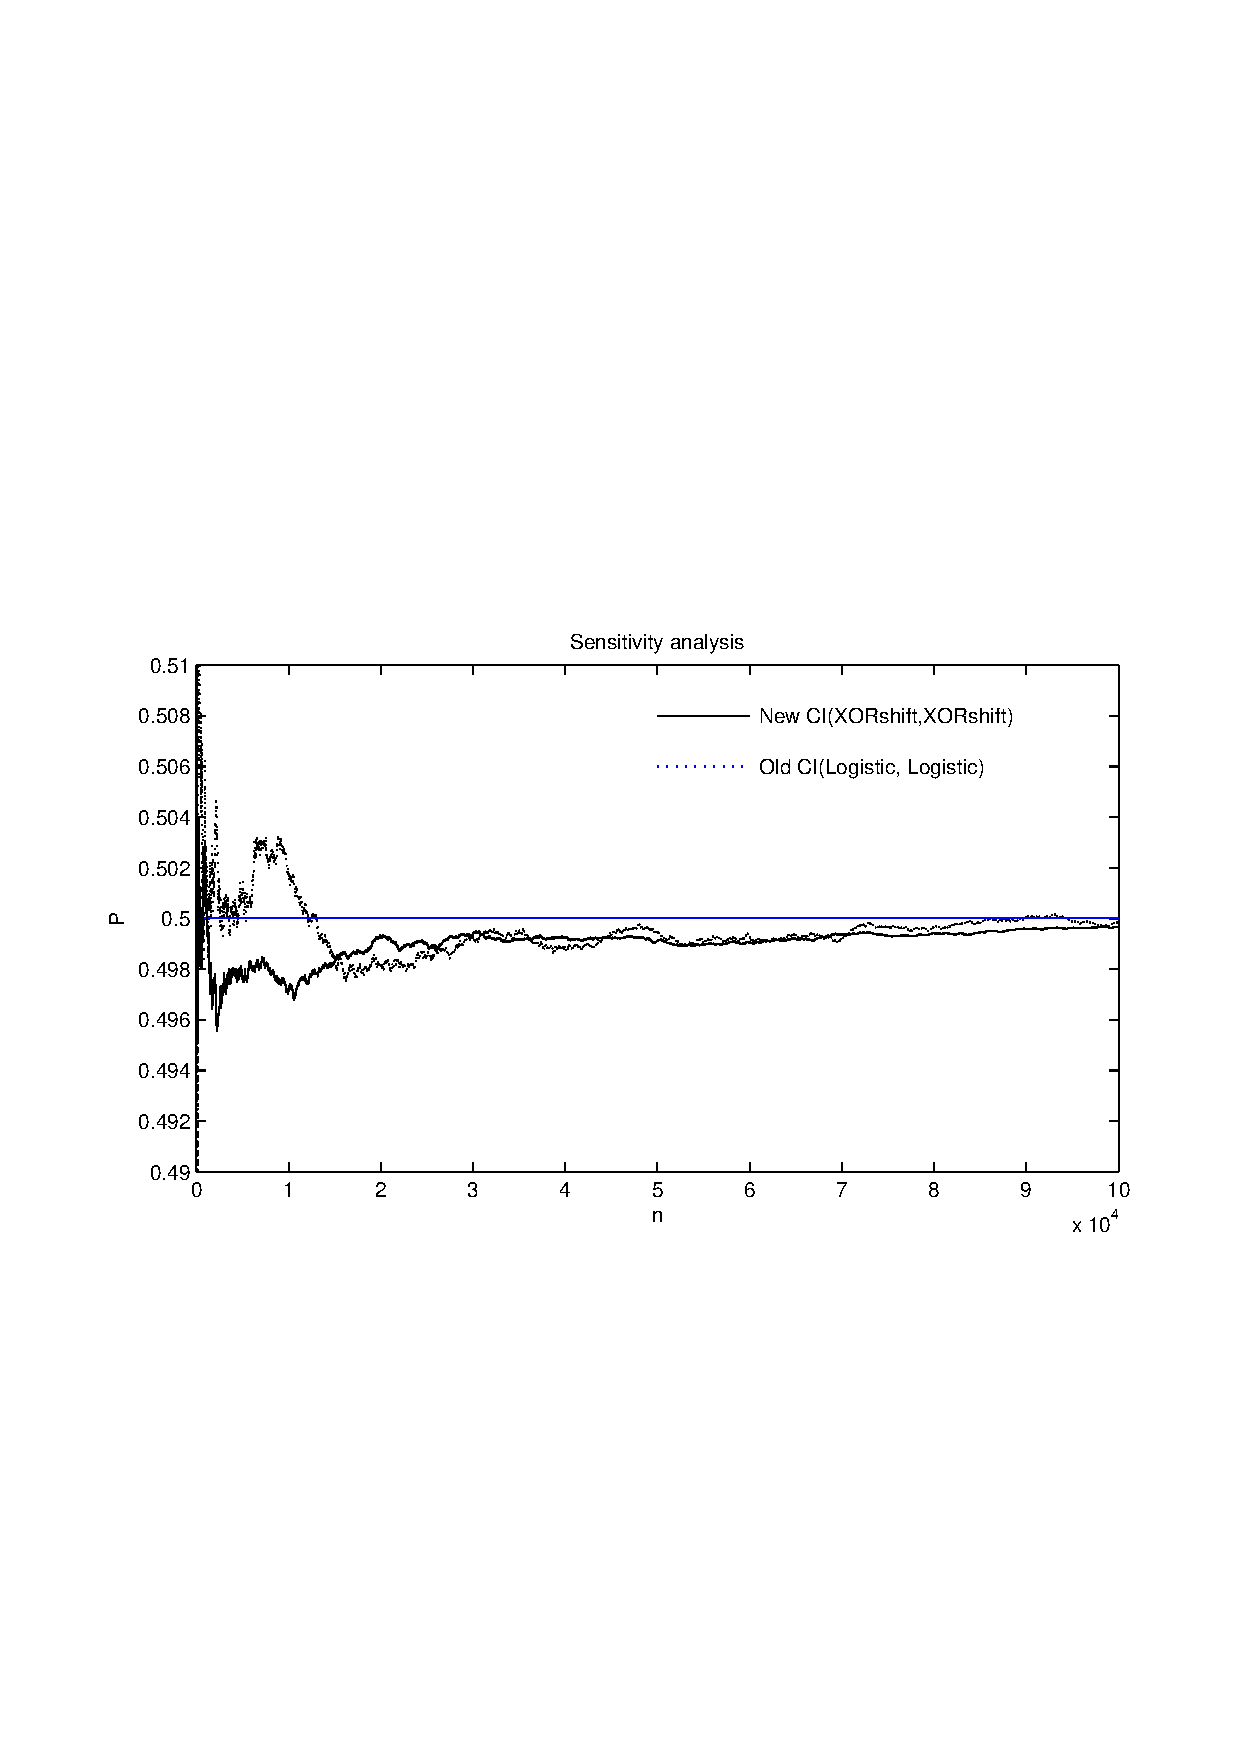
\includegraphics[width=3.5in]{comparative_sensitivity2.pdf}
% \DeclareGraphicsExtensions.
% \caption{Sensitivity analysis}
% \label{Sensitivity analysis}
% \end{figure}



% \subsubsection{Uniform distribution}

Figure~\ref{fig:SecondOrderDistribution} gives a 3D graphic representation of the distribution of a random sequence obtained by our generator. The point cloud presents a uniform distribution that tends to fill the complete 3D space, as expected for a random signal. To obtain this cloud, we have first changed the binary sequence to a $N$-bit integer sequence $x_1$, $x_2$, $x_3$, $x_4$... Then we have plot $\left(\frac{x_1}{2^N},\frac{x_2}{2^N},\frac{x_3}{2^N}\right), \left(\frac{x_2}{2^N},\frac{x_3}{2^N},\frac{x_4}{2^N}\right)$...


\begin{figure}[h!] 
\centering
\subfigure[Sensitivity]{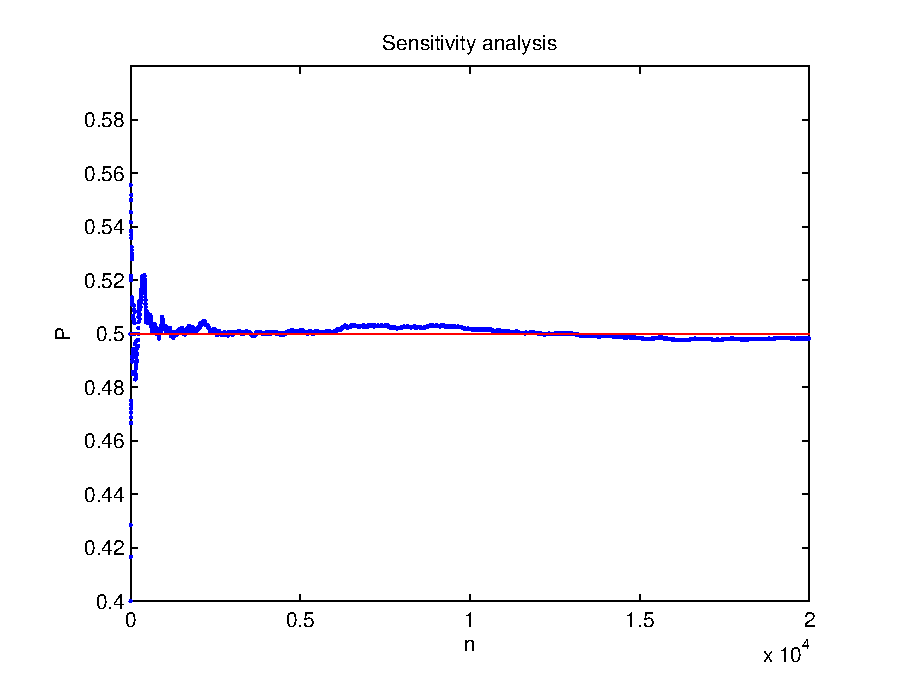
\includegraphics[width=4.2cm]{Sensitivity_analysis_xx2.eps}
\label{fig:Sensitivity}}
\subfigure[Second order distribution]{\includegraphics[width=4.2cm]{Second_order_distribution.eps}
\label{fig:SecondOrderDistribution}} 
\caption{Security analysis}
\label{SecurityAnalysis}
\end{figure}


% \subsubsection{Auto-correlation and cross-correlation}

The PRNGs adopted in this section is Scheme 6.
The auto-correlation and cross-correlation of the symbolic sequence are respectively given in Figures~\ref{fig:autocorrelation} and \ref{fig:crosscorrelation}. It can be seen that this sequence has $\delta$-like auto-correlation which is required for a good PRBNG. The sequences generated with different initial values will have zero cross-correlation due to the sensitive dependence on initial conditions.



\begin{figure}[h!] 
\centering
\subfigure[Auto-correlation]{\includegraphics[width=4.2cm]{autorcorrelation.eps}
\label{fig:autocorrelation}}
\subfigure[Cross-correlation]{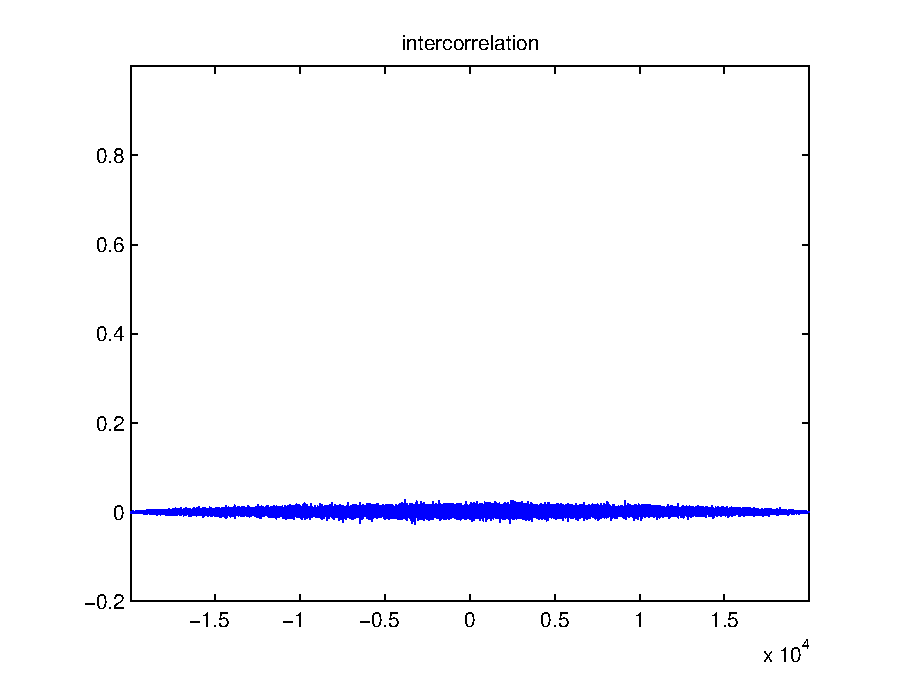
\includegraphics[width=4.2cm]{intercorrelation.eps}
\label{fig:crosscorrelation}} 
\caption{Auto and cross-correlation of the pseudo-random sequence}
\label{The auto-correlation &The cross-correlation of the pseudo-random sequence}
\end{figure}

% \subsubsection{Linear complexity}

The linear complexity (LC) of a sequence is the size in bits of the shortest linear feedback shift register (LFSR) which can produce this sequence. This value measures the difficulty of generating -- and perhaps analyzing -- a particular sequence.
Indeed, the randomness of a given sequence can be linked to the size of the smallest program that can produce it. LC is the size required by a LFSR to be able to produce the given sequence. The Berlekamp-Massey algorithm can measure this LC, which might be used to evaluate the ``security'' of a pseudo-random sequence.
It can be seen in Figure~\ref{Linear complexity} that the LC curve of a sample sequence of 2000 b is close to the ideal line $C_i=i/2$, which implies that the generator has high linear complexity. 

% \begin{figure}
% \centering
% \includegraphics[width=2.5in]{linear_complexity_new_ci.eps}
% \DeclareGraphicsExtensions.
% \caption{Linear complexity}
% \label{Linear complexity}
% \end{figure}

% \subsubsection{FFT}

The FFT of the sequence (Figure.~\ref{The FFT of the pseudo-random sequence}) is performed and the corresponding power spectrum is computed. A complete flat power spectrum, with almost equal frequency contribution for all frequencies, is indicative of a total random series.

% \begin{figure}[!t]
% \begin{center}
% \begin{tabular}{c}
% 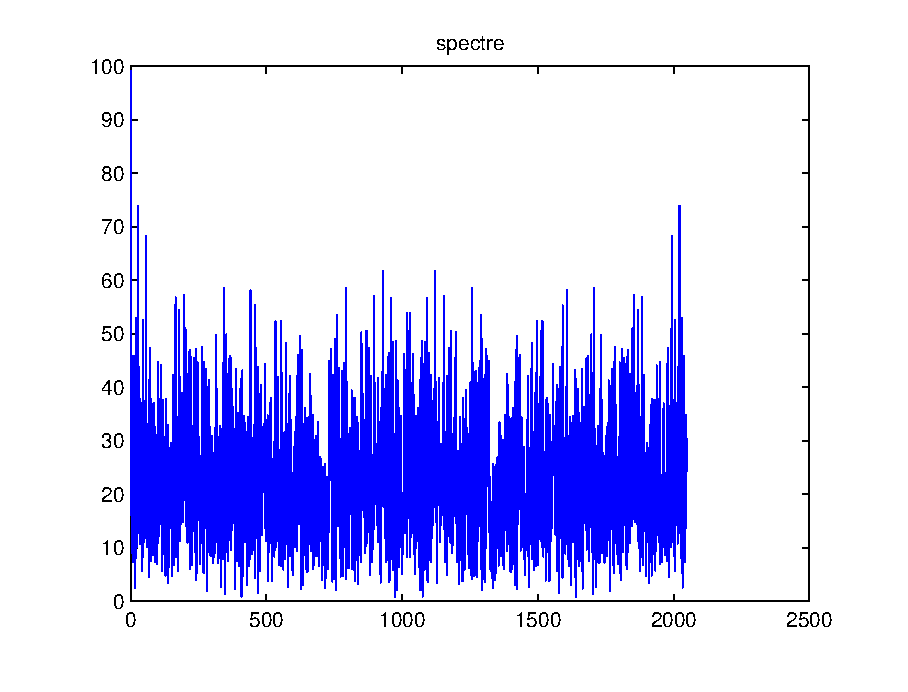
\includegraphics[width=2.5in]{spectre.eps}  \\ 
% % \emph{Fig 3} The FFT of the pseudo-random sequence\\
% \end{tabular}
% \caption{The FFT of the pseudo-random sequence}
% \label{The FFT of the pseudo-random sequence}
% \end{center}
% \end{figure}

\begin{figure}[h!] 
\centering
\subfigure[Linear complexity]{\includegraphics[width=4.2cm]{linear_complexity_new_ci.eps}
\label{Linear complexity}}
\subfigure[FFT]{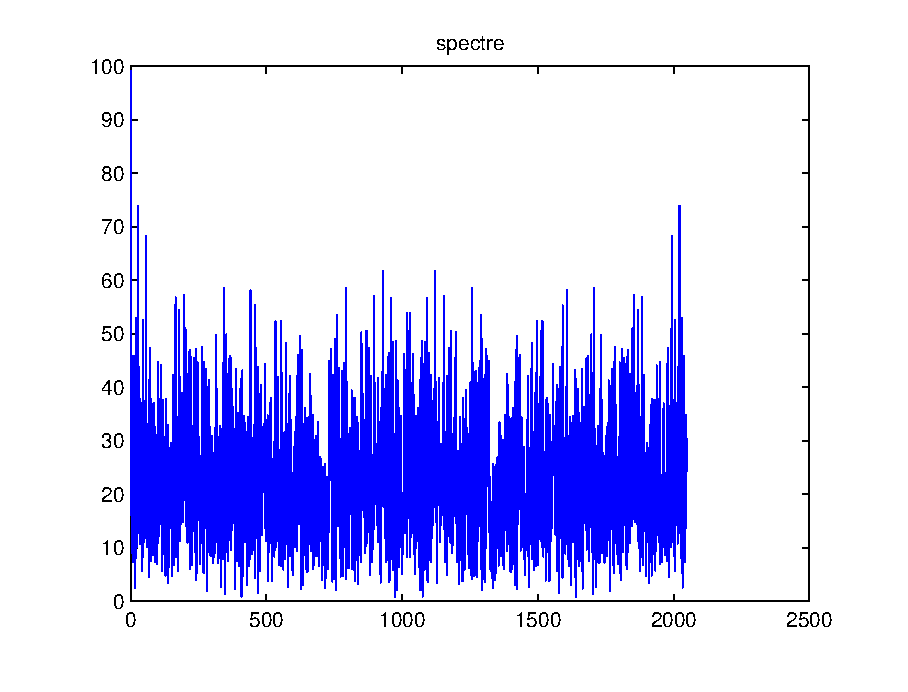
\includegraphics[width=4.2cm]{spectre.eps}
\label{The FFT of the pseudo-random sequence}} 
\caption{The Linear complexity and FFT of the pseudo-random sequence}
\label{The Linear complexity and FFT of the pseudo-random sequence}
\end{figure}

\subsection{Devaney's chaos property}

Generally, the quality of a PRNG depends, to a large extent, on the following criteria: randomness, uniformity, independence, storage efficiency, and reproducibility. A chaotic sequence may satisfy these requirements and also other chaotic properties, as ergodicity, entropy, and expansivity. A chaotic sequence is extremely sensitive to the initial conditions. That is, even a minute difference in the initial state of the system can lead to enormous differences in the final state, even over fairly small timescales. Therefore, chaotic sequence fits the requirements of pseudo-random sequence well. Contrary to XORshift, our generator possesses these chaotic properties~\cite{guyeux10},\cite{wang2009}.
However, despite a large number of papers published in the field of chaos-based pseudo-random generators, the impact of this research is rather marginal. This is due to the following reasons: almost all PRNG algorithms using chaos are based on dynamical systems defined on continuous sets (\emph{e.g.}, the set of real numbers). So these generators are usually slow, requiring considerably more storage space and lose their chaotic properties during computations. These major problems restrict their use as generators~\cite{Kocarev2001}.

In this paper we don't simply integrate chaotic maps hoping that the implemented algorithm remains chaotic. Indeed, the PRNG we conceive is just discrete chaotic iterations and we have proven in \cite{guyeux10} that these iterations produce a topological chaos as defined by Devaney: they are regular, transitive, and sensitive to initial conditions. This famous definition of a chaotic behavior for a dynamical system implies unpredictability, mixture, sensitivity, and uniform repartition. Moreover, as only integers are manipulated in discrete chaotic iterations, the chaotic behavior of the system is preserved during computations, and these computations are fast.
%Generally, the success of a PRNG study depends, to a large extent, on the following criteria:
%uniformity, independence, storage efficiency, reproducibility. Chaotic sequence
%has not only these good pseudo-random characteristics but also chaotic properties,
%as ergodicity, entropy and expansivity. It is extremely sensitive to the initial states. That is, even a minute
%difference in the starting state of the
%system can lead to enormous differences in the final state of the system even over
%fairly small timescales. Therefore, chaotic sequence well fits the requirements of
%pseudo-random sequence.\newline
%Despite a huge number of papers published in the field of chaos-based pseudo-random generators, the impact that this research has made on conventional cryptography is rather marginal. This is due to the following reasons: almost all chaotic algorithms are based on dynamical systems defined on the set of real numbers. So these generators are usually slow, require considerably more storage space and lose their chaotic property during computations. These major problems restrict their use in cryptography~\cite{Kocarev2001}.\newline
%The generator proposed in this paper does not inherit its chaotic properties from a real chaotic map, but from chaotic iterations defined in Section \ref{subsection:Chaotic iterations}. It has been proved in~\cite{guyeux10} that chaotic iterations behave as chaos, as it is defined by Devaney: they are regular, transitive and sensitive to initial conditions. This most famous definition of a chaotic behavior for a dynamical system implies unpredictability, mixture, sensitivity
%and uniform repartition. The principal interest is that chaotic iterations don't use real numbers.
%This allows the creation of a new generation of chaotic pseudo-random number generators. Because only integers are manipulated in chaotic iterations, the chaotic behavior of the system is preserved during computations, and these computations are fast.

